\documentclass[a4paper,twoside, openright,12pt]{report}
\usepackage{psfrag,amsbsy,graphics,float}
\usepackage[dvips]{graphicx, color}
\usepackage[latin1]{inputenc}
\usepackage{verbatim} 
\usepackage{appendix}

% MY CHANGE
%\usepackage[bookmarksnumbered=true]{hyperref} 

\usepackage[bookmarks=true,colorlinks=true,       % false: boxed links; true: colored links
    linkcolor=black,          % color of internal links
    citecolor=black,        % color of links to bibliography
    filecolor=black,      % color of file links
    urlcolor=black           % color of external links
]{hyperref}
 

%%% Stand 14.09.2007
%%% erstellt von Marion Sobotka
%%% marion.sobotka@tum.de
%%% last changes: 14.01.09


%_______Kopf- und Fu�zeile_______________________________________________________
\usepackage{fancyhdr}
\pagestyle{fancy}
%um Kopf- und Fu�zeile bei chapter-Seiten zu reaktivieren
\newcommand{\helv}{%
   \fontfamily{phv}\fontseries{a}\fontsize{9}{11}\selectfont}
\fancypagestyle{plain}{	
	\fancyfoot{}% keine Fu�zeile
	\fancyhead[RE]{\helv\leftmark}% Rechts auf geraden Seiten=innen; in \leftmark stehen \chapters
	\fancyhead[LO]{\helv\rightmark}% Links auf ungeraden Seiten=au�en;in \rightmark stehen \sections
	\fancyhead[RO,LE]{\thepage}}%Rechts auf ungeraden und links auf geraden Seiten
%Kopf- und Fu�zeile f�r alle anderen Seiten
\fancyfoot{}
\fancyhead[RE]{\helv\leftmark}
\fancyhead[LO]{\helv\rightmark}%alt:\fancyhead[LO]{\itshape\rightmark}
\fancyhead[RO,LE]{\thepage}
%________________________________________________________________________________


%_Definieren der R�nder und L�ngen__________
\setlength{\textwidth}{15cm}
\setlength{\textheight}{22cm}
\setlength{\evensidemargin}{-2mm}
\setlength{\oddsidemargin}{11mm}
\setlength{\headwidth}{15cm}
\setlength{\topmargin}{10mm}
\setlength{\parindent}{0pt} % Kein Einr�cken beim Absatz!!
%___________________________________________


%_______Titelseite__________________________________________
\begin{document}
\pagestyle{empty}
\enlargethispage{4.5cm} %Damit das Titelbild weit genug unten ist!
\begin{center}
\phantom{u}
\vspace{0.5cm}
\Huge{\sc Numerical Test Rig for Large-Scale and Interconnected Dynamical
Systems}\\
\vspace{1.5cm}
                                 \large{submitted\\
				  Project Laboratory\\
				  Networked and Cooperative Control\\
			  %DIPLOMARBEIT\\%/STUDIENARBEIT/MASTERRBEIT/BACHELORARBEIT\\ 
                               %            von\\
                              %  \large{Zwischenbericht zur\\
			%DIPLOMARBEIT/STUDIENARBEIT/MASTERARBEIT/
					   % BACHELORARBEIT\\ 
					   by         

						
					\begin{tabular}{c c}
					    \vspace{0.4cm} & \vspace{0.4cm} \\
					 cand. ing. Francisco Llobet& cand. ing. Jose Rivera  \\
						\vspace{0.5cm} & \vspace{0.5cm}\\
					born on December 18, 1986 & born on December 18, 1986\\
					resident: & resident:\\
					Amalienstr. 87& Amalienstr. 87\\
					80799 M\"{u}nchen & 80799 M\"{u}nchen  
					\end{tabular}

					                           
					%Tel.: +49\,176\,233\,14721\\
					\vspace{1.5cm}
					Institute of\\
					Automatic Control Engineering\\
					Technische Universit\"{a}t M\"{u}nchen\\
					\vspace{0.3cm}
					Univ.-Prof. Dr.-Ing./Univ. Tokio Martin Buss\\
                                        Univ.-Prof. Dr.-Ing. Sandra Hirche}
\end{center}
\vspace{2.5cm}
\begin{tabular}{ll}
Supervisor: & F. Deroo, S. Erhart, A. Gusrialdi, H. Mangesius  \\
Beginn: & 09.05.2011  \\
Submitted &  04.07.2011 \\
\end{tabular}
%____________________________________________________________

\newpage

%_______Abstract_____________________________________________
\topmargin5mm
\textheight220mm
\pagenumbering{arabic}
\phantom{u}
\begin{abstract}
The goal of this project was to develop a test rig for large-scale and interconnected dynamical systems. The result was 
MTIDS or Matlab Toolbox for Interconnected Dynamical Systems, which is a mashup that wraps different toolboxes used for graph analysis and 
dynamic systems simulations together. MTIDS allows the definition and analysis of Graphs, where each node has a user defined behavior  
%\vspace{2cm}
% \begin{center}
% \normalsize \textbf{Zusammenfassung}\\
% \end{center}
% Dieser Hauptseminar besch\"{a}ftigt sich mit der Methode der getriggerten Optimierung. Dabei wird besonderen Focus auf die m\"{o}glichen Anwendungen f\"{u}r Energiesystemen gesetzt.
% Als erstes wird eine Analyse der Methode in ihre genaralisierte Form f\"{u}r das NUM (Netzwerk Nutzen Maximirung) Problem durchgef\"{u}hrt. Als zweites wird ihre Anwendung an das OPF (Optimale Leistungsfluss) in Energienetzen evaluiert. Als letztes werden
% verbesserungs Vorschl\"{a}gen und weitere Anweundungen in Energiesystemen diskutiert.  
\end{abstract}
%____________________________________________________________

\newpage

%_______Widmung_______________________________________________
\phantom{u}
\phantom{1}\vspace{6cm}
\begin{center}
%Hier die Widmung oder leer lassen
\end{center}
%_____________________________________________________________



\pagestyle{fancy}

%_________Inhaltsverzeichnis__________________________
\tableofcontents 
%_____________________________________________________




%_________Einleitung__________________________________
\chapter{Introduction} \label{chapter1}



\begin{figure}[htb]
\centering
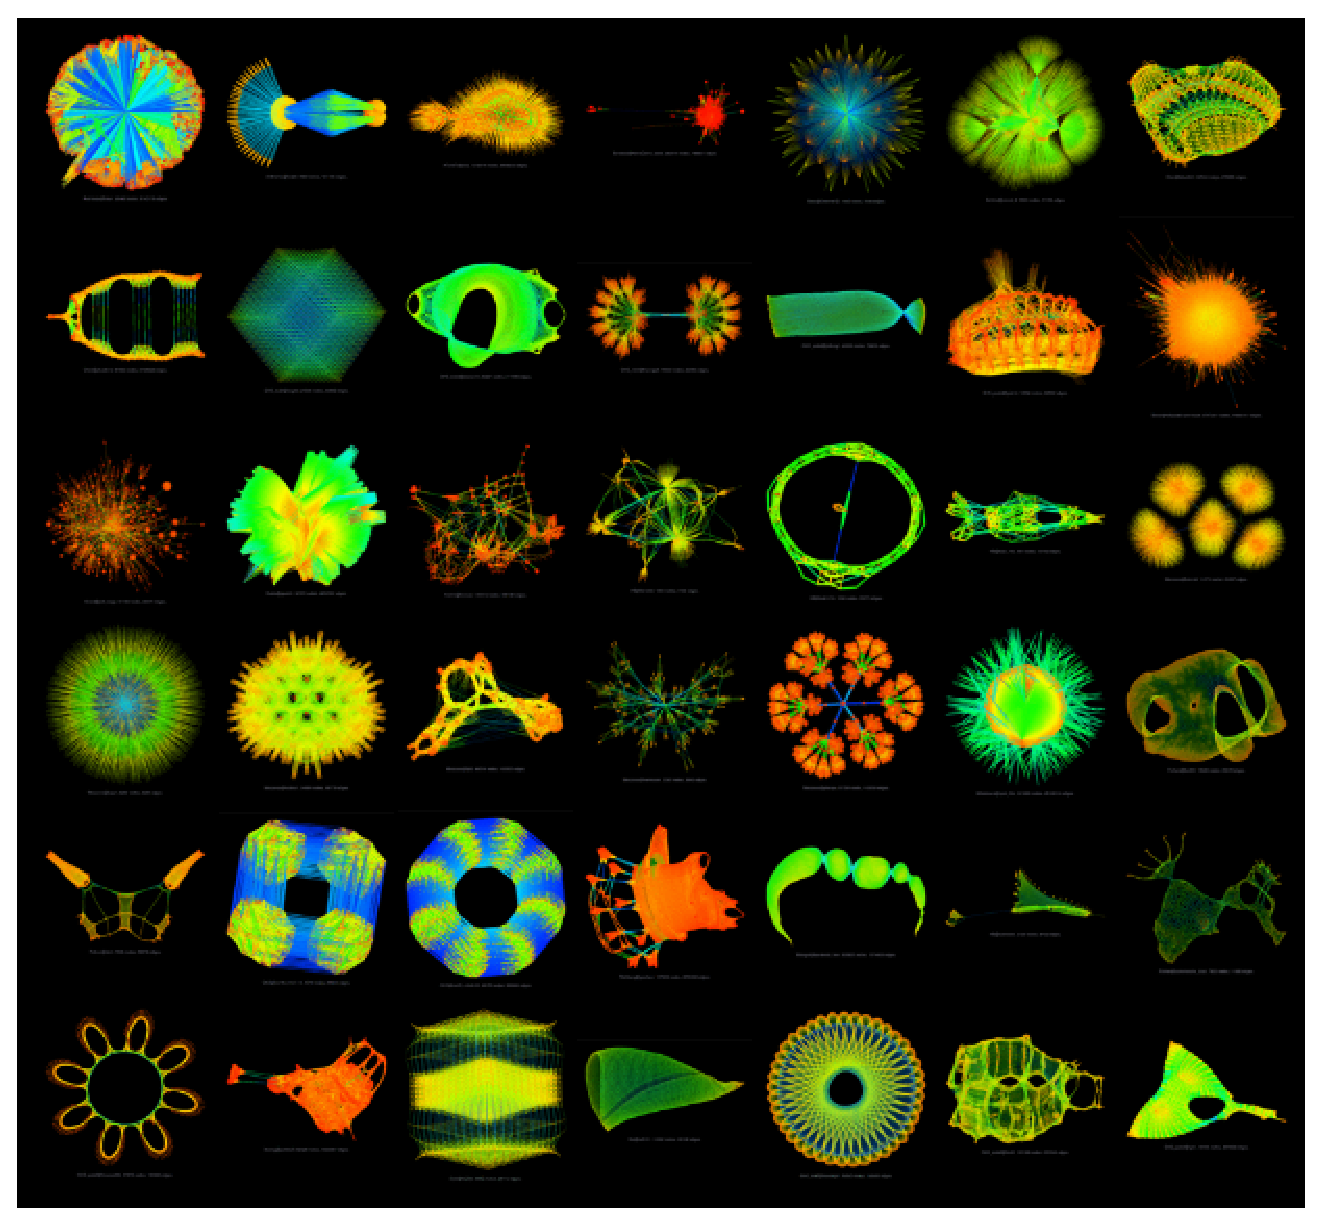
\includegraphics[width=0.5\textwidth]{pics/complex.eps}
\caption[write text]{write text}
\label{modelNormal1}
\end{figure}



\begin{figure}[htb]
\centering
\includegraphics[width=0.5\textwidth]{pics/mtidsstructure.eps}
\caption[write text]{write text}
\label{modelNormal1}
\end{figure}



\begin{figure}[htb]
\centering
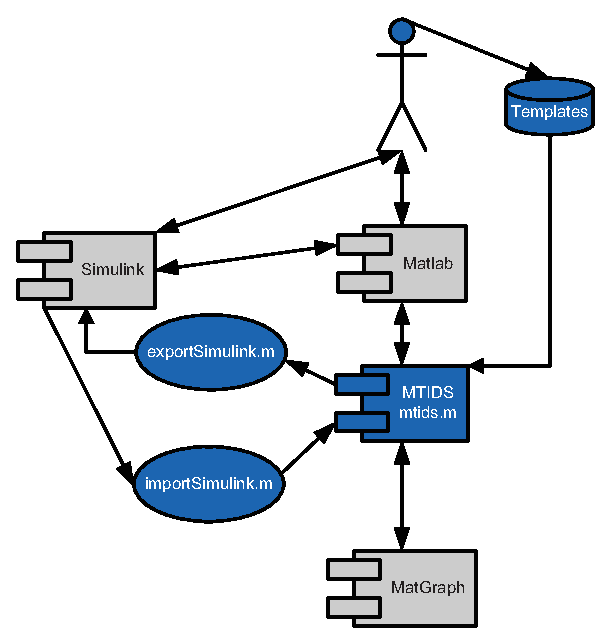
\includegraphics[width=0.5\textwidth]{pics/uml.eps}
\caption[write text]{write text}
\label{modelNormal1}
\end{figure}

\chapter{Graphic Theory Tools}\label{chapter2}

%%%%%%%%%%%%%%%%%%%%%%%%%%%%%%%%%%%%%%%%%%%%%%%%%	CONCLUSION	%%%%%%%%%%%%%%%%%%%%%%%%%%%%%%%%%%%%%%%%%%%%%%%%%%%%%%%%%%%%%%%%%%%%%%%


%______________________________________
\chapter{System Theory Tools}\label{chapter3}



\chapter{Conclusion and Future Development}
\section{Conclusion}


\section{Future Development}
%
%_______________________________________________________________


%_____Abbildungsverzeichnis_________________________________
\cleardoublepage
\addcontentsline{toc}{chapter}{List of Figures} 
\listoffigures 	 %Abbildungsverzeichnis

%___________________________________________________________
% 
% %_____Literaturverzeichnis_________________________________
% \cleardoublepage
% \addcontentsline{toc}{chapter}{Bibliography}
% \bibliography{bibliography.bib}
% \bibliographystyle{alpha}
% %__________________________________________________________


%________________Appendix_____________________________________________%


\end{document}
